\documentclass[12pt,a4paper]{book}
\usepackage[top=1.5cm,bottom=3cm,left=1cm,right=1cm]{geometry}
\usepackage{graphicx}
\usepackage{times,multicol,microtype}
\usepackage{lipsum}
\parindent0pt
\begin{document}
\sffamily
\fboxrule1pt
\pagestyle{empty}
\mbox{}
\centerline{\huge\bfseries CAPE OF GOOD HOPE}
\vskip2\baselineskip
%\fbox{\scalebox{1}{\hbox{\vbox{%

\leavevmode\hbox{\vtop{\hsize.35\textwidth\bfseries\Large\sffamily\noindent DEVELOPMENT OF\\ POSTAL SERVICES}}\hfill
\leavevmode\hbox{\hsize0.35\textwidth\vtop{\bfseries\Large\sffamily  INSTRUCTIONAL\\MARKINGS }}


\vfill
\fboxrule0pt
\centering

\framebox{\begin{minipage}{1\textwidth}
\centering
\bfseries\large ADVERTIZED AND UNCLAIMED MARK
\end{minipage}}
\vfil
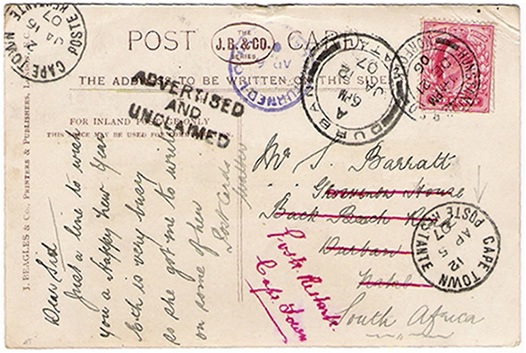
\includegraphics[width=\textwidth]{./images/Advertized-and-Unclaimed-postmark}\par
\hfill Ex-Goldblatt

\vfill


\centering
\framebox{\begin{minipage}{0.8\textwidth}
%\begin{multicols}{3}
\leavevmode
  1864 wrapper P.O.  Saron to cape Town light blue “On Service” outer letter sheet from the tiny mission station at Saron with top backflap opened and showing a fine “double arc” cancel of Saron dated “DE 20 1864” addressed to the Postmaster General at Cape Town bearing in addition town oval transit in red on bottom backflap, Tulbagh “DE 20 1864” plus Cape Town arrival on address panel, opened out for display, an extremely rare postmark. 1864 wrapper P.O.  
%\end{multicols}
\end{minipage}}



%}}}}
\end{document}